\chapter{Theory}
\section{Artificial Neural Networks}
\paragraph{Why Neural Networks?}
Before going into what actually artificial neural networks are, let's first
try to face the question why do we need it in this paper. The problem that
we give to our application to solve can be shortly summarized in the following statement:
\blockquote{
Given a group of images, find the patterns in them that are more influential
on your belief that an image(or a group of images) belongs to a specific class.
}


% Given a group of images, find the patterns in this images
% that will change or influence on your belief more than other patterns
% that an image or a group of images belongs to a specific class.
}
This is problem is known as pattern recognition problem or in our case
visual pattern recognition problem \cite{Bishop1995}.
The solve this problem it's required to develop ability for a machine
to recognize patterns that will help to make a decision about a class.
The obstacles that can appear by solving this problem can be more visible
if we will try to write a conventional computer program, i.e. bunch of rules
to identify these patterns. What seems to be easy for us, is really hard to describe
algorithmically. In these system the computational steps are deterministic
hence not flexible enough for the whole variety of input data \cite{Nielsen2015}.

\subparagraph{Solving problem differently}
Artificial Neural Networks(and machine learning in general) are looking at the problem
in a different way.
They don't execute programs instructions, they don't have
sequential semantic and normally are not
deterministic. They acquire their "knowledge" by extracting patterns from raw data,
which normally called training data(which normally is a set of tuple \code(input, label))
This approach also know as concept of statistical pattern recognition. \cite{Bishop1995}
Artificial Neural networks have recently shown an excellent performance and
accuracy at recognizing objects compared with other
machine learning techniques \cite{Krizhevsky2012}.

\paragraph{What is Neural Network?}
Artificial Neural Network(ANN), often referred just as Neural Network(NN),
in simply words is a computational model, which was inspired by how human/animal
brain works. Artificial NN is modeled based on the neuronal structure in the brain's
cortex. Though the inspiration was from the brain,
it's indeed much much simpler than brain in terms of number of neurons that is used
in ANN \cite{Goodfellow-et-al-2016}.
To understand how neural networks works it is crucial to understand first the
way perceptron work, which is simple type of an artificial neuron.
Given several binary inputs, perceptron is meant to produce a single binary output.
\begin{figure}[H]
	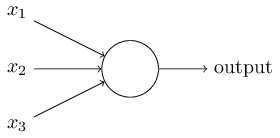
\includegraphics[width=\linewidth]{perceptron.png}
	\caption{A perceptron.} % to show under the picture
	\label{igm:model} % to reference to the figure later
\end{figure}
In the figure \ref{igm:model} the perceptron has three inputs: $x_1, x_2, x_3$.

% The problem that we trying to solve in this paper is known as
% pattern recognition problem. We trying to recognize pattern in images
% in order. The problem can be described
% as searching for patterns in data like image, text, sound and etc. An example
% of the problem can be to find a tree in a picture.

% What is special about? desribe few properties of neural network
% differencet between Conventional algoritms
% what else is usable for



 \cite{rosenblatt1962principles}
% \subparagraph{} What is meant here by computation.
\subparagraph{Perceptron}


% biases weights
% - shortly how it works, a simple example but clear example. Better about MNIST data.
% ona layer network
% multi layer network

\paragraph{Basic concept of neural network}
There are a good variety of
explain the example in terms of the elements
layers, activation function. How output is produce.

- about learning weights/ parameters , about data. Ground truth.

- write shortly about how one updates parameters. About stoschastic gradient descent

- different activation functions
- learning rate
- a little bit about backpropagation.
